\documentclass[a4paper,twosides,openright,titlepage]{book}
\usepackage[italian,english]{babel}
\usepackage[ autostyle,italian=guillemets]{csquotes}
\usepackage[bibstyle=numeric,backend=biber]{biblatex}
\addbibresource{bibliography.bib}

\usepackage{frontespizio}
\usepackage{etoolbox}
\usepackage[Bjornstrup]{fncychap}


\preto\chapter{\raggedright}
\usepackage{microtype,amsmath,booktabs,graphicx,fancyhdr,listings,xcolor,multirow,wrapfig,hyperref}
\usepackage[section]{placeins}

\newenvironment{abstract}% 
	{\cleardoublepage%
		\thispagestyle{empty}% 
		\null \vfill\begin{center}%
		\bfseries \abstractname \end{center}}% 
	{\vfill\null}

\definecolor{mygray}{rgb}{0.28,0.28,0.28}
\lstset{%frame=tb,
  xleftmargin=\parindent,
  language=C,
  backgroundcolor = \color{lightgray},
  commentstyle=\color{mygray},
  aboveskip=3mm,
  belowskip=3mm,
  showstringspaces=false,
  columns=flexible,
  basicstyle={\small\ttfamily},
  numbers=none,
  breaklines=true,
  breakatwhitespace=true,
  tabsize=4
  %xleftmargin = 2cm
}
\setcounter{tocdepth}{4}
\setcounter{secnumdepth}{4}

\begin{document}

\begin{frontespizio}
\makeatletter
\begin{Preambolo*}
\usepackage{etoolbox}
\makeatletter
\patchcmd{\preparefrontpagestandard}
  {\if\@front@{logo} 
   \includegraphics[height=\front@logosize]{\front@logo}\par
   \vspace{\frontlogosep}
   \fi}
  {}
  {}{}
\patchcmd{\preparefrontpagestandard}
  {\if\@front@{school}
   \front@school
   \else
   Corso di \front@cl
   \fi}
  {Corso di \front@cl
  \par\if\@front@{logo}
   \vspace{4\frontlogosep}
   \includegraphics[height=\front@logosize]{\front@logo}\par
   \vspace{\frontlogosep}
   \fi
  }{}{}
\makeatother
\end{Preambolo*}
\makeatother
\Istituzione {POLITECNICO DI MILANO}
\Logo[6.5cm]{grafici/logo_Polimi} 
\Divisione{Scuola di Ingegneria Industriale}
\Corso [Laurea Magistrale]{Ingegneria Aeronautica }
\Titolo {Scaling Performance of a DNS \\
 solver written in CPL}
\Candidato{{Mirco Meazzo\\  873477}}
\Relatore {Prof. Maurizio Quadrio}
%\NCorrelatore {Relatore esterno}{Relatori esterni}
\Correlatore{ ...}
\Annoaccademico {2018-2019}
\end{frontespizio} 

\frontmatter
\selectlanguage{english}
\graphicspath{grafici}

\begin{flushright} 
\null\vspace{\stretch{1}}
\pagestyle{empty}
\par Dedicata alla mia famiglia,\par a chi mi ha sempre sostenuto, \par a chi è presente oggi \par e a chi non c'è più
\vspace{\stretch{2}}\null
\end{flushright}




\begin{abstract}
\hrulefill

A numerical method for the direct numerical simulation of the incompressible Navier–Stokes equations in rectangular geometries is presented. The method implement the MPI Standard~\cite{MPI} to the engine developed by M.~Quadrio and P.~Luchini described in~\cite{cpl:presentazione}. 

The method is based on Fourier expansions in the homogeneous directions and fourth-order accurate, compact finite-difference schemes over a variable-spacing mesh in the wall-normal direction. 

Two different versions of the solver have been developed, based on the domain decomposition.  In the first the domain is decomposed through 1D (\emph{Slab}), while in the second version 2D (\emph{Pencil}) decomposition is used.
The performances of these versions have been compared against each other.

To manage the decomposition we rely on the APIs present in \emph{fftMPI}, developed by Steve Plimpton at Sandia National Laboratories~\cite{fftMPI}.
\\
\\
\\
\emph{Key words}: Navier–Stokes equations, direct numerical simulation, parallel computing, turbulence, 2D decomposition, pencil 

\hrulefill
\end{abstract}




\tableofcontents 
\listoffigures 
\listoftables



\mainmatter
\chapter{Introduction}
\section{Problem Definition}
\pagestyle{headings}

Before moving to what has been done in this thesis I wish to briefly discuss the setup of our channel flow and the equations used to solve the problem.

We have the domain sketched in figure~\ref{sketch_dominio} where the $x$ and $z$ coordinates denote the streamwise and spanwise directions of the flow, while the $y$ coordinate is the wall normal ones.
Along these three dimension we have $u,v$ and $w$ components of velocity.

The flow is assumed to be periodic in the streamwise and spanwise directions. The lower wall is at position $y_l$ and the upper wall at position $y_u$. The reference length $\delta$ is taken to be one half of the channel height.
Once an appropriate reference velocity is chosen, we can define the Reynolds number as:
\[
Re = \frac{U\delta}{\nu}
\]
where $\nu$ is the kinematic viscosity of the fluid.

According to our geometry and the assumption of incompressible flow, we can express the behavior of the flow through the mass conservation law and the Navier-Stokes equations, which in a dimensionless form states:\\
\begin{equation}
\frac{\partial u}{\partial x} + \frac{\partial v}{\partial y} + \frac{\partial w}{\partial z};
\label{mass:cons}
\end{equation}
\begin{subequations}
\label{eqn:schema}
\begin{align}
\frac{\partial u}{\partial t} + u\frac{\partial u}{\partial x} + v\frac{\partial u}{\partial y} + w\frac{\partial u}{\partial z} &= 
- \frac{\partial p}{\partial x} + \frac{1}{Re} \nabla^{2}u;  \\
\frac{\partial v}{\partial t} + u\frac{\partial v}{\partial x} + v\frac{\partial v}{\partial y} + w\frac{\partial v}{\partial z} &= 
- \frac{\partial p}{\partial y} + \frac{1}{Re}\nabla^{2}v;\\
\frac{\partial w}{\partial t} + u\frac{\partial w}{\partial x} + v\frac{\partial w}{\partial y} + w\frac{\partial w}{\partial z} &= 
- \frac{\partial p}{\partial z} + \frac{1}{Re}\nabla^{2}w;
\end{align}
\end{subequations}

\begin{figure}
\centering
\includegraphics[width=0.8\textwidth]{grafici/sketch_dominio}
\caption{Domain of interest}
\label{sketch_dominio}
\end{figure}


the engine of Quadrio and Luchini described into~\cite{cpl:presentazione} which works per \emph{y-slabs}, as shown in figure~\ref{domain_decomp},
\begin{figure}
\centering
\includegraphics[width=0.5\textwidth]{grafici/decomp_dominio_cpl}
\caption{Original domain decomposition in case of 4 processors}
\label{domain_decomp}
\end{figure} allowing to perform the convolutions and relatives Fourier transformations locally on each processor, leading to a minimum of communication, moving to communication intensive decompositions, such as \emph{z-slabs}, \emph{x-slabs} or \emph{pencils}.

These solutions require communication to perform the array transpose needed by the FFTs in the two homogeneous directions
\chapter{Code Structure}
\section{Spatial discretization along homogeneous directions}
Our solver is based on a Fourier approach. Among the advantages of such approach we face the possibility to expansion of the unknown functions in terms of truncated Fourier series in the homogeneous directions. For example the wall-normal component $v$ of the velocity vector is represented as:
\begin{equation}
v(x,y,z,t) = \sum_{h=-nx/2}^{+nx/2} \sum_{l=-nz/2}^{+nz/2} \hat{v}_{hl}(y,t) e^{i\alpha x}e^{i \beta z}
\end{equation}
where:
\begin{equation}
\alpha = \frac{2\pi h}{L_{x}} = \alpha_{0} h; \quad \beta= \frac{2 \pi l}{L_{z}} = \beta_{0}l
\end{equation}

$h$ and $l$ are integer indexes corresponding to the streamwise and spanwise direction respectively, and $\alpha_{0}$ and $\beta_{0}$ are the fundamental wavenumbers in these directions, defined in terms of the streamwise and spanwise lengths $L_{x} = {2\pi}/{\alpha_{0}} $ and $L_{z} = {2 \pi}/{\beta_{0}}$ of the computational domain. The computational parameters given by the streamwise and spanwise lenght of the computational domain, $L_{x}$ and $L_{z}$ , and the truncation of the series, $nx$ and $nz$, must be chosen so as to miminize computational errors. For further details regarding the proper choice of a value of $L_{x}$ see~\cite{QuadrioMaurizio2003Issi}.

The convolutions required to solve the equations~\ref{curl:momentum:y} and~\ref{normal:velocity} are computationally expensive if carried out in the frequency domain. The same evaluation can be performed efficiently by first transforming the three Fourier components of velocity back in physical space, multiplying them in all six possible pair combinations and eventually retransforming the results into the Fourier space. Fast Fourier Transform algorithms are used to move from Fourier to physical space and viceversa. The aliasing error is removed by expanding the number of modes by a factor of at least $3/2$ before the inverse Fourier transforms, to avoid the introduction of spurious energy from the high-frequency into the low-frequency modes during the calculation.



\section{Finite difference scheme}


\subsection{Compute of the finite difference coefficients}




\section{Time Discretization}





\section{Domain Decompositions}
The engine of Quadrio and Luchini described into~\cite{cpl:presentazione} works per \emph{y-slabs}, as shown in figure~\ref{domain_decomp},
\begin{figure}
\centering
\includegraphics[width=0.8\textwidth]{grafici/decomp_dominio_cpl}
\caption{Original domain decomposition in case of 4 processors}
\label{domain_decomp}
\end{figure}
 allowing to perform convolutions and Fourier transformations locally on each processor, avoiding the cost of non-local transposition for the velocity array and the non-linear terms ones. Such implementation, denominated pipelined-linear-system (PLS), lead to a minimum of communication, in fact this approach require to send and receive only the values stored in the two upper and lower boundary cells of the local decomposition, in order to provide the data required by the fourth-order finite difference scheme.
 \par
 Using the PLS approach the number of bytes exchanged in a three step Range-Kutta method are:
 \begin{equation}
 D_{t} = 3 \times 8 \times (p-1) \frac{3}{2} \times \frac{nx}{p} \frac{nz}{p} \times ny \times 18
 \label{exchange:data:cpl}
 \end{equation}
 where:
 \begin{description}
  \item[3] takes into account the number of time steps;
  \item[8] for counting the bytes;
  \item[$\mathbf{(p-1)}$] is the number of nodes across which the exchange take place;
  \item[ $\mathbf{\frac{3}{2}}$ ] corresponds to the expansion in horizontal modes required by the dealiasing process;
  \item[ $\mathbf{\frac{nx}{p} \times \frac{nz}{p}}$] is the grid portion, for each plane, to exchange with the others nodes;
  \item[18] due to the 3 velocities plus the 6 products to be exchanged twice, before and after the FFT;
  \item[ny] takes into account the number of planes to be exchanged.
\end{description}
Further details about the PLS communications are available in \cite[\nopp chapter 4.2]{ns:quadrio}. \\
 \par
Although efficient for small processors grid, the performances of this approach falls quickly whether the processors number becomes comparable with \emph{ny}.  Furthermore the code structure limit the number of parallel process to be just a fraction of the \emph{ny} extension.
\par
To avoid such limitations and increase the number of parallel processes we decided to move from PLS approach to something different.
We have identified two possible solutions:
\begin{description}
  \item employ \textbf{slab} decomposition along x or z axis;
  \item employ \textbf{pencil} decomposition.
\end{description}
Both implementation require extensive use of the MPI paradigm and, possibly, a library to handle such decompositions.
We opted to employ OpenMPI\cite{openmpi} for what concern the MPI paradigm, in particular we entrust to the well established OpenMPI version 3.1, release 3.1.3.
The ideas behind the choice of such library rely on the fact the OpenMPI is released behind BSD license\cite{bsd:license}, it is designed to group different MPI implementation, avoiding fragmentation and forking problem\cite{faq:openmpi} and, although less optimized on proprietary fabric such as Intel Omni-Path fabric\cite{intel:omnipath}\cite{intel:intelmpivsopenmpi}, is wider spread.


 while, for the decomposition, we entrusted in a new library, released by the 


\subsection{Slabs decomposition}


\subsection{Pencil decomposition}


%\section{Parallel I/O}

Input-output could be a serious bottleneck if we do not pay the right attention.
In particular, when dealing with supercomputers, two major problems arise:
\begin{itemize}
\item needing of parallel I/O,
\item avoid endianness problem related.
\end{itemize}
As first thing let us introduce I/O.\par
\begin{wrapfloat}{figure}{l}{0pt}
\includegraphics[width=0.5\textwidth]{grafici/masterslave}
\caption{Master-Slaves I/O setup}
\end{wrapfloat}
In computer architecture, the combination of the CPU and main memory, to which the CPU can read or write directly using individual instructions, is considered the brain of a computer. Any transfer of information to or from the CPU/memory combo, for example by reading data from a disk drive, is considered I/O~\cite{io}.
When dealing with cluster the transit of data from disk to CPU is not so straightforward. The presence of multiple CPU require the adoption of one of the following strategies.\par
The most basic strategy is the master-slaves setup. In this kind of strategy a single node of the grid have access to the storage, therefore no scalability is provided. The slave nodes must send/receive data from the master, therefore we face strong slowdown related to the huge workload required to perform I/O by the single node and the following communications among nodes.\par
A second approach is shown here beside and consist in performing distributed I/O on local files. Such kind of implementation is scalable, ensure data consistency and avoid communication during I/O phase. 
\begin{wrapfloat}{figure}{r}{0pt}
\includegraphics[width=0.5\textwidth]{grafici/localio}
\caption{Distributed I/O on local files}
\end{wrapfloat}However, since every processor writes data on its own hard storage, it require a great deal of post processing work to glue data among each others, which increase linearly with the number of processes. For this reason we can not consider it affordable. \\
\begin{wrapfloat}{figure}{r}{0pt}
\includegraphics[width=0.5\textwidth]{grafici/mpiio}
\caption{Coordinated controlled accesses}
\end{wrapfloat}
\par
The last kind of I/O setup, which is the most updated and optimized, is the so called coordinated controlled accesses.
Scalability reaches its peak with this kind of implementation, which takes care of possible communications needing by its own.
In this approach every CPU can access to the single storage memory in which the dataset is hosted, and in concomitancy with the other processes, writes the data. As can be understood, the reading/writing operation is intrinsically fragile, since guarantee data consistency can be hard. To avoid consistency lacks, the MPI-IO has been introduced with the deployment of MPI-2 standard~\cite{MPI:standard2}.

On top of MPI-IO several high level I/O libraries arose, two well established examples are parallel netCDF and parallel HDF5. 

At exception of the master-slave approach, every presented strategy require the adoption of a parallel file system.
In computing, a file system or filesystem controls how data is stored and retrieved. Without a file system, information placed in a storage medium would be one large body of data with no way to tell where one piece of information stops and the next begins. By separating the data into pieces and giving each piece a name, the information is easily isolated and identified. We can briefly define the file system as the structure and logic rules used to manage the groups of information and their names.
In the same fashion a parallel file system maintains logical space and provides efficient access to data for distributed memory configurations.\\
\par
Let us establish the concept of endianness.
Intel introduces their white paper with the following sentence:\par
``Endianness describes how multi-byte data is represented by a computer system and is dictated by the CPU architecture of the system. Unfortunately not all computer systems are designed with the same Endian-architecture. The difference in Endian-architecture is an issue when software or data is shared between computer systems''\cite{endianness}.\par
Since our binary database has been built on Marconi, at Cineca, but the post-processing analysis take place on our personal computers, we need to guarantee results portability with a reliable method to store the data. \\
\par
Unfortunately MPI-IO can not set a bit ordering different from the machine's natives ones, and we can not assure portability in this way. To do so we have to move from MPI-IO to a library capable to satisfy our requirements.\par
Employ the well established parallel HDF5 library is the natural choice.





\chapter{Code Benchmarks}
\section{Scaling Performance of $128^3$ problem}
\pagestyle{headings}


\section{Scaling Performance of $256^{3}$ problem}
The medium sized problem shows better scaling performances compared to the small ones.
This behavior, in which bigger problems provide better scaling capabilities, has been highlighted and discussed by many authors in past.
After a little preamble about scaling let us dig into results.\\
\par
A slab decomposed algorithm provide gains of $\mathcal{O}(10)$ in terms of execution times, less than a pencil decomposed algorithm, but with better results for small processors grid. In fact, as depicted in figure~\ref{1281} the 1D decomposition curve achieve lower execution times than the 2D ones, until 8 cores.\\
Passed 8 cores the pencil decomposition prevails, reaching speedup factors above 100, with time savings in the order of magnitude of $\mathcal{O}(100)$ with respect to the single core runtime.
In the figure~\ref{1283} is possible to see the efficiencies achieved by the two methods, running on 64 threads per processor. It is important to denote the behavior of the pencil decomposed algorithm, which, until 8 cores in use, exhibits high scaling efficiency.
Passed 8 cores, to recover high efficiency we must decrease the number of threads per processor.
\section{Scaling Performance of $512^3$ problem}
Let us proceed now showing the performances achieved by our code in a medium sized problem.
The present simulation shown a better scaling effectiveness and efficiency for both methods with respect to $128^{3}$ problem. 
\par
Once again the best results are reached using 64 cores per processor, possibly indicating that the array dimension fits in the cache memory.
\par
The speedup peak is remarkable, with a factor of $260$ on $2048$ cores using pencil decomposition, while stops around $38$ using $128$ cores and slab decomposition. \\
\par

\begin{figure}
\begin{center}
\includegraphics[scale=0.6]{grafici/5121}
\caption{Scaling performance of $512^3$ simulation}
\label{5121}
\end{center}
\end{figure}

\begin{figure}
\begin{center}
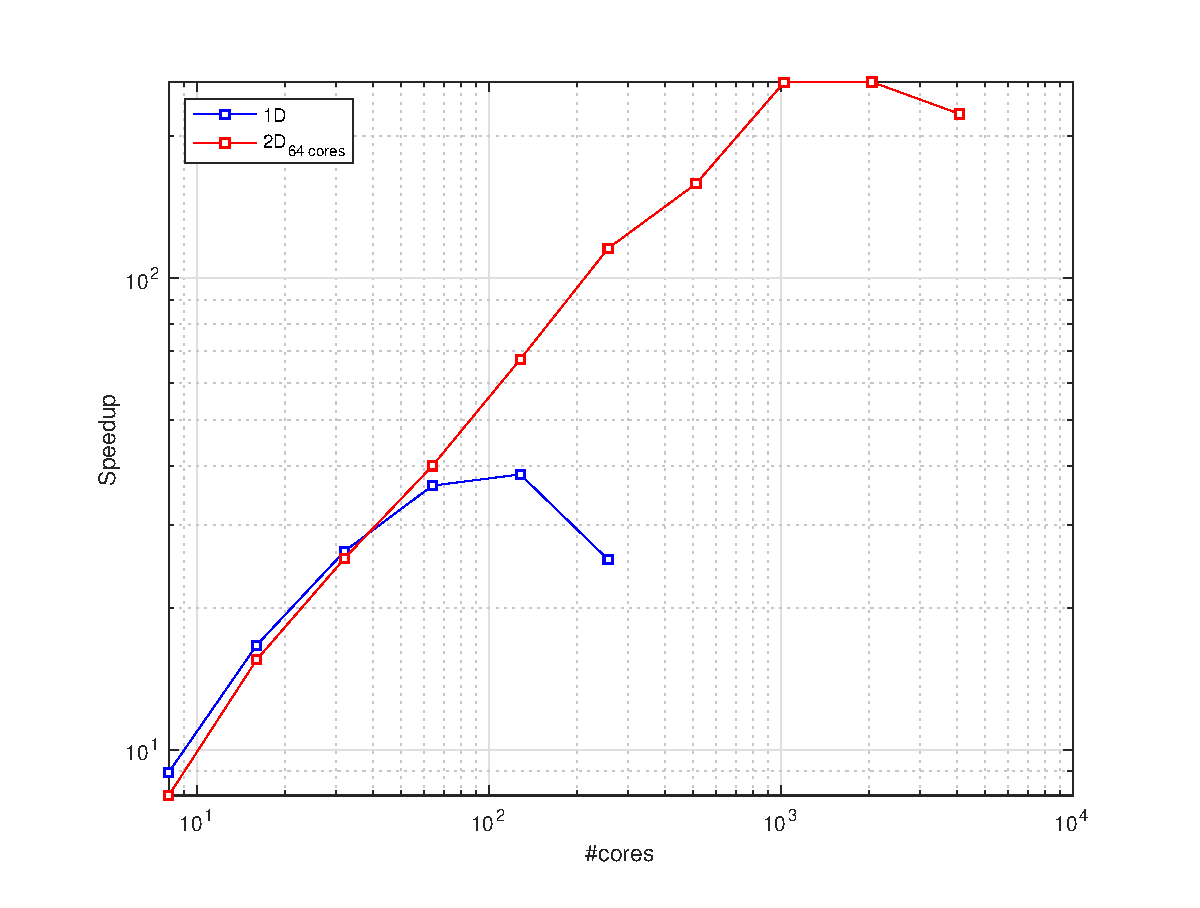
\includegraphics[scale=0.6]{grafici/5122}
\caption{Speedup performance factor of $512^3$ simulation}
\label{5122}
\end{center}
\end{figure}

As we can see from figure~\ref{5122}, the speedup factor of the 2D decomposed algorithm increase approximately linearly until $256$ cores. The raise in performance continue at lower factor until $1024$ cores are reached, where nearly stops before start descending once passed $2048$ cores.
The inverse behavior is shown in figure~\ref{5121}, where the simulation time is plotted against the number of cores.\\
In figure~\ref{5121} is also reported the theoretical scaling limit. Comparing this line, in dashed green, with our results let us conclude that our scaling, although linear for the majority of the time, is sub-optimal. 
The same reasoning is valid also for the slab decomposed algorithm, although in a smaller region of cores number.
It is interesting to denote the advantageous behavior of such algorithm until $64$ cores, where both performances are still slightly different in terms of speedup factor. 
\par
By looking at the values in table~\ref{512data} of page~\pageref{512data} and the depicted counter part, in figures~\ref{5121} and \ref{5122}, it is possible to denote that between $8$ and $16$ cores the loss are really small. This lead us to expect a perfect theoretical linear behavior from $1$ to $16$ cores. Keeping this in mind, we feel confident and seems reasonable to consider a speedup factor of $8$ for the $8$ cores simulation, possibly doing an error below the unit. \\
\par
We refer to figure~\ref{5123} to have an idea of the efficiency of the algorithm. The figure shows that the efficiency remains above $80\%$ until $32$ cores are used. However, once passed such limit, the behavior is linear and smoother with respect to the ones shown in figure~\ref{644} of page~\pageref{644}.

\begin{figure}
\begin{center}
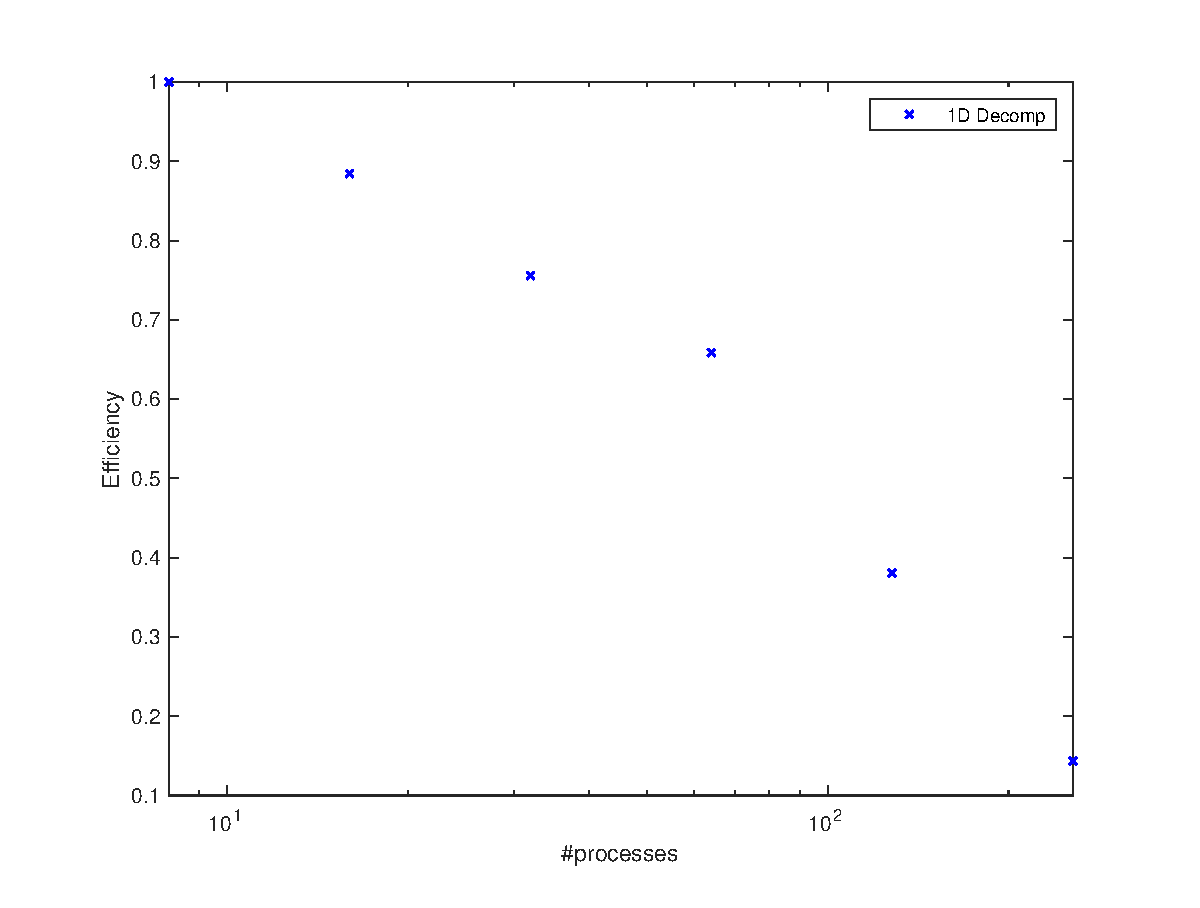
\includegraphics[scale=0.6]{grafici/5123}
\caption{Efficiency factor of $512^3$ simulation}
\label{5123}
\end{center}
\end{figure}


\begin{table}[h]
\caption{Data from $512^{3}$ simulation, if present first row indicates 1D decomposition}
\begin{center}
\begin{tabular}{c c c c}
\toprule
\textbf{\#cores} & \textbf{Time [s]} & \textbf{Speedup} & \textbf{Efficiency [\%]} \\
\midrule
\multirow{2}{*}{8} & 1750 & 8.96 & 112 \\
& 1960 & 1 & 100 \\
\hline
\multirow{2}{*}{16} & 941.5 & 16.65 & 104 \\
& 1011 & 15.51 & 97 \\
\hline
\multirow{2}{*}{32} & 595.3 & 26.35 & 82 \\
& 616.2 & 25.45 & 80 \\
\hline
\multirow{2}{*}{64} & 432.1 & 36.3 & 57 \\
& 392.3 & 39.97 & 62 \\
\hline
\multirow{2}{*}{128} & 409.2 & 38.34 & 30 \\
& 233.2 & 67.22 & 53 \\
\hline
\multirow{2}{*}{256} & 620.1 & 25.29 & 10 \\
& 135.7 & 115.5 & 45 \\
\hline
512 & 99 & 158.4 & 31 \\
1024 & 60.4 & 259.6 & 25 \\

\bottomrule
\end{tabular}
\end{center}
\label{512data}
\end{table}%
\section{Scaling Performance of $4096\times512\times256$ problem}
The last benchmark deal with very large problems. Like for the previous large problem, the dimensions are so huge to require the adoption of multiple processors to run, otherwise we will face an out of memory error.
On a Intel Xeon Phi~\cite{intel:xeonphi} the minimum requirements are to employ at least 2 processors and use 32 cores, or less, per processor.
\par
As the previous problem have highlighted, the less cores are used and the better results are scored, so our impossibility to go further than 32 cores per processor, as pointed some rows before, would not be a big deal. We may suppose that the poorest results will be achieved by 32 cores runs, instead of the 64 ones. \\
\par

\begin{figure}
\begin{center}
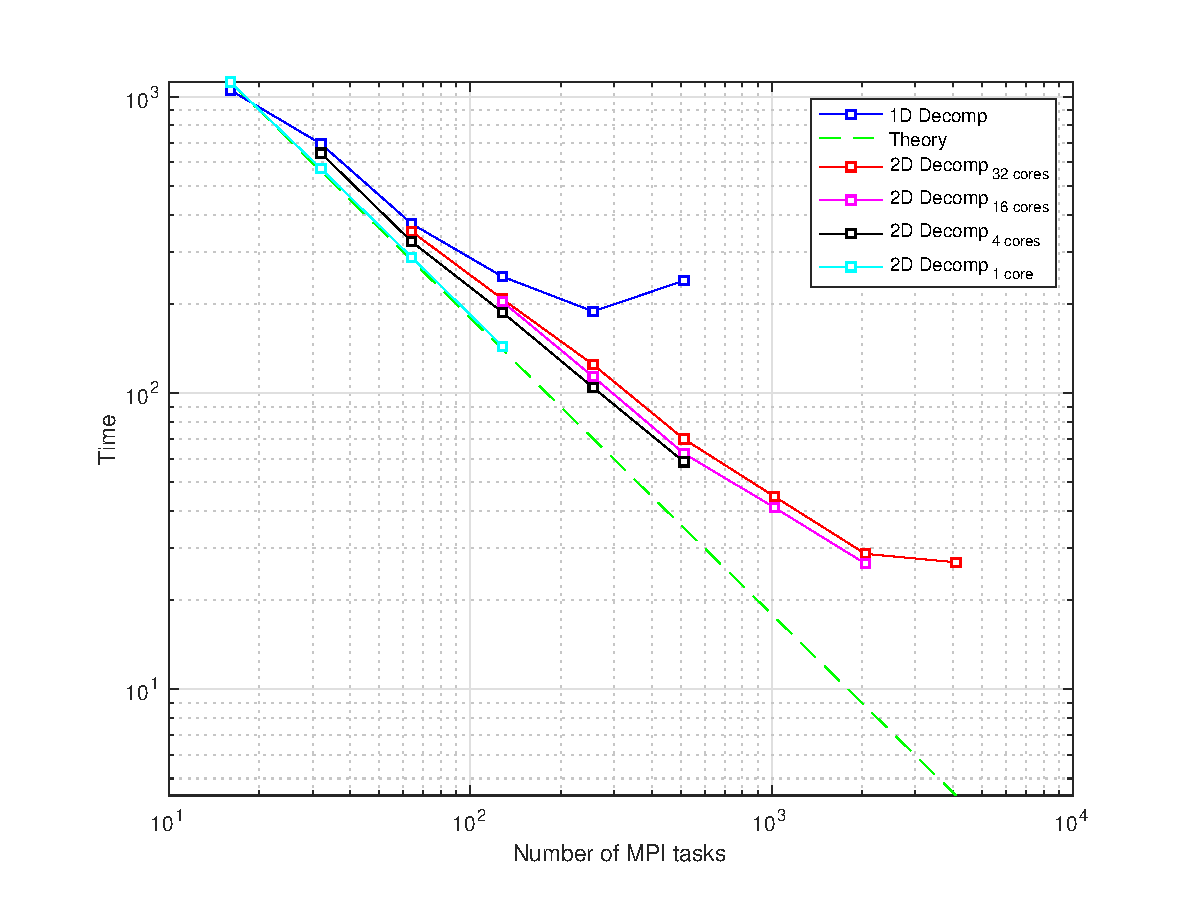
\includegraphics[scale=0.6]{grafici/20481}
\caption{Time scaling comparison for $4096\times 512\times 256$ simulation}
\label{20481}
\end{center} 
\end{figure}

Let us start showing figure~\ref{20481} in which is reported the time scaling of our code.\par
As could be seen, the 2D decomposition using single core achieved the lowest timing execution.
It is interesting to denote how this combination fits the theoretical behavior perfectly.\par
All other 2D decomposed combinations exploit a worse behavior with respect to the single core run, with a marked trend, where the increase in cores per processor number leads to poorer performances. \par 
Such behavior is aligned with our predictions.\\

\begin{figure}
\begin{center}
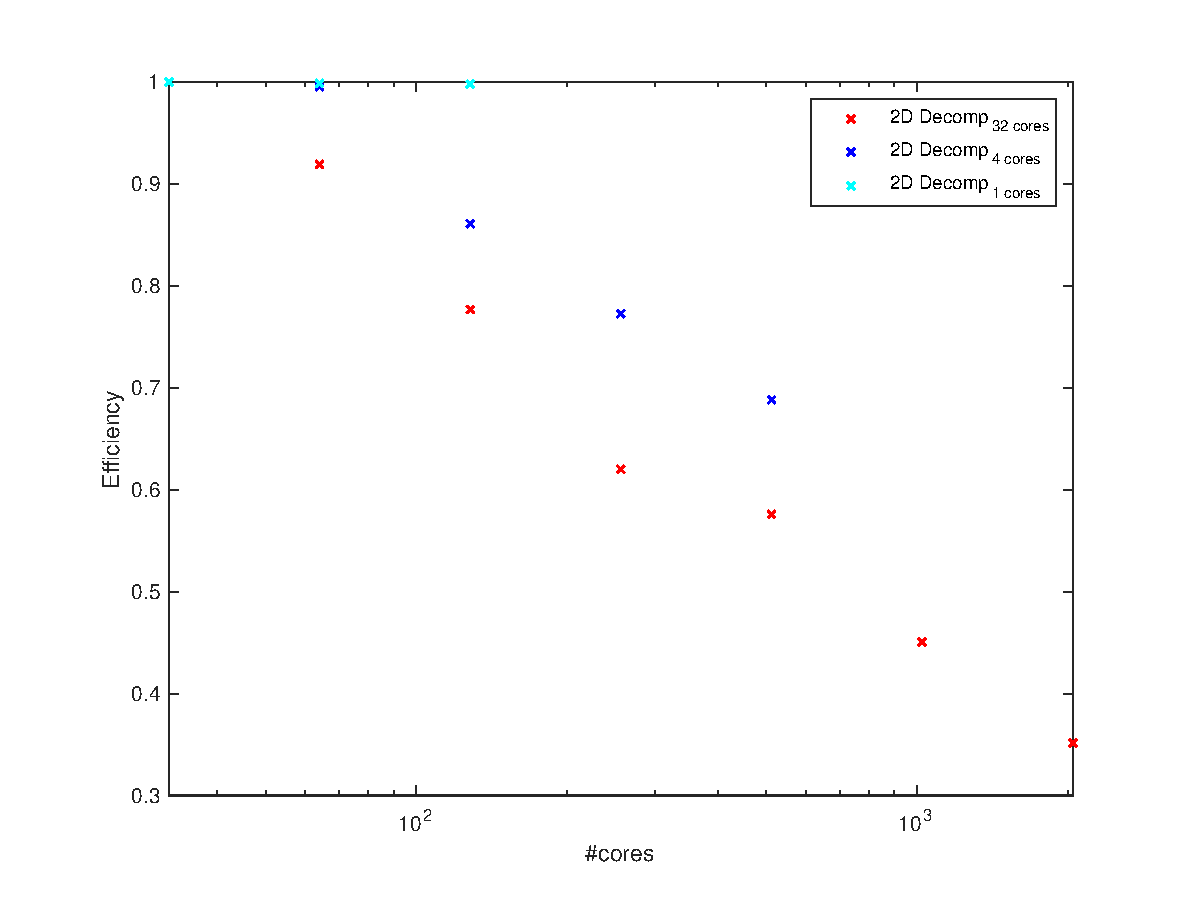
\includegraphics[scale=0.6]{grafici/20483}
\caption{Efficiency factor of $4096\times512 \times256$ simulation using 1D decomposition}
\label{20483}
\end{center}
\end{figure}

\begin{table}
\caption{Data from $4096\times 512\times 256$ simulation, 1D decomposition}
\begin{center}
\begin{tabular}{c c c c}
\toprule
\textbf{\#Processes} & \textbf{Time [s]} & \textbf{Speedup} & \textbf{Efficiency [\%]}\\
\midrule
16 & 1052.9 & 16 & 100\\
32 & 693 & 24.31 & 76\\
64 & 372.5 & 45.23 & 71\\
128 & 247 & 68.2 & 53\\
256 & 188.5 & 89.37 & 35\\
512 & 239.5 & 70.34 & 14\\
\bottomrule
\end{tabular}
\end{center}
\label{2048:data:1}
\end{table}

\par
For what concern about the 1D decomposed algorithm, which, since the code structure is slightly different, can run also on 64 cores per processor, it achieve the worst performances among all possible solutions, highlighting once again the benefits of using a pencil decomposed approach. \par
The speedups achieved by this kind of domain decomposition can be seen in table~\ref{2048:data:1}, on page~\pageref{2048:data:1}, while the efficiency graph, which shows a poor behavior, can be seen in figure~\ref{20483}. \\
\par



Far more interesting, are the data in table~\ref{2048:data:2}, which report the speedups, efficiency and timing achieved by the algorithm with 2D decomposition. The data, and the graphical counterpart which can be seen on page~\pageref{20482} in figure~\ref{20482} and~\ref{20484}, report a very high efficiency using single core, while, although smaller, a still high efficiency is preserved by using 4 cores per processor.\\
\par
\begin{figure}
\begin{center}
\includegraphics[scale=0.6]{grafici/20484}
\caption{Efficiency factor of $4096\times512 \times256$ simulation using 2D decomposition}
\label{20484}
\end{center}
\end{figure}
Increasing the counter of threads per processor leads to constant losses, as expectable. However, such losses between adjacent stations are lower than the ones of the previous simulations, furthermore we can see wider gaps among the efficiency curves, symptom that there is wider room for improvements.\par
Moreover, at very high number of cores, the efficiency curves slope is minor than before, preserving efficiency and allowing us to perform faster computations with greater speedups.\\
\par
To talk about speedups is useful to introduce figure~\ref{20482}, in which these are reported.\par
The graph, on page~\pageref{20482}, shows the results achieved by the 1D and 2D domain decomposed algorithm, with emphasis on the effects of the variation of cores per processor quantity, for the 2D algorithm only.\par
As has been done in the previous section, the high efficiency shown by the single core run, combined with the physical impossibility to use less cores, has lead us to made the assumption of speedup equal to 16 for a 16 parallel processes run in a single core environment.All other efficiencies and speedups have been derived using such data as reference.\\
\par

\begin{table}
\caption{Data from $4096\times 512\times 256$ simulation, 2D decomposition}
\begin{center}
\begin{tabular}{c c c c c}
\toprule
\textbf{\#Processes} & \textbf{Time [s]} & \textbf{Speedup} & \textbf{Efficiency [\%]} & \textbf{cores}\\
\midrule
16 & 1121.5 & 16 & 100 & 1\\
\hline
\multirow{2}{*}{32} & 571.4 & 31.4 & 98 & 1\\
& 644.8 & 27.83 & 87 & 4\\
\hline
\multirow{3}{*}{64} & 287.2 & 62.47 & 98 & 1\\
& 323.9 & 55.39 & 87 & 4\\
& 350.7 & 51.17 & 80 & 16\\
\multirow{4}{*}{128} & 143.8 & 124.8 & 98 & 1\\
& 187.2 & 95.85 & 75 & 4\\
& 203.4 & 88.23 & 69 & 16\\
& 207.5 & 86.47 & 68 & 32\\
\hline
\multirow{3}{*}{256} & 104.3 & 172 & 67 & 4\\
& 113.4 & 158.2 & 62 & 16\\
& 124.6 & 144 & 56 & 32\\
\hline
\multirow{3}{*}{512} & 58.6 & 306.4 & 60 & 4\\
& 62.5 & 287.1 & 56 & 16\\
& 70 & 256.5 & 50 & 32\\
\hline
\multirow{2}{*}{1024} & 41 & 437.5 & 43 & 16\\
& 44.7 & 401.4 & 39 & 32\\
\multirow{2}{*}{2048} & 26.6 & 675.5 & 33 & 16\\
& 28.7 & 626.3 & 31 & 32\\
\hline
4096 & 26.8 & 668.8 & 16 & 32\\
\bottomrule
\end{tabular}
\end{center}
\label{2048:data:2}
\end{table}

As can be seen in table~\ref{2048:data:2} the best result is achieved using 16 cores per processor and 2048 parallel processes. Unfortunately, due to some policy limitations, we can not push forward our resources request, although the graph clearly shows margins of improvements for such configuration.\\
\par
Differently from all the previous simulations, the processor grid for the pencil decomposition results balanced when the streamwise stencil has half the modes with respect to the other direction. Such configuration has been suggested by benchmarks.
\par
In conclusion we may say that, although the modes distribution results unbalanced in this simulation, the speedup trend still remain aligned with the ones exhibited in the other simulations.
\begin{figure}
\begin{center}
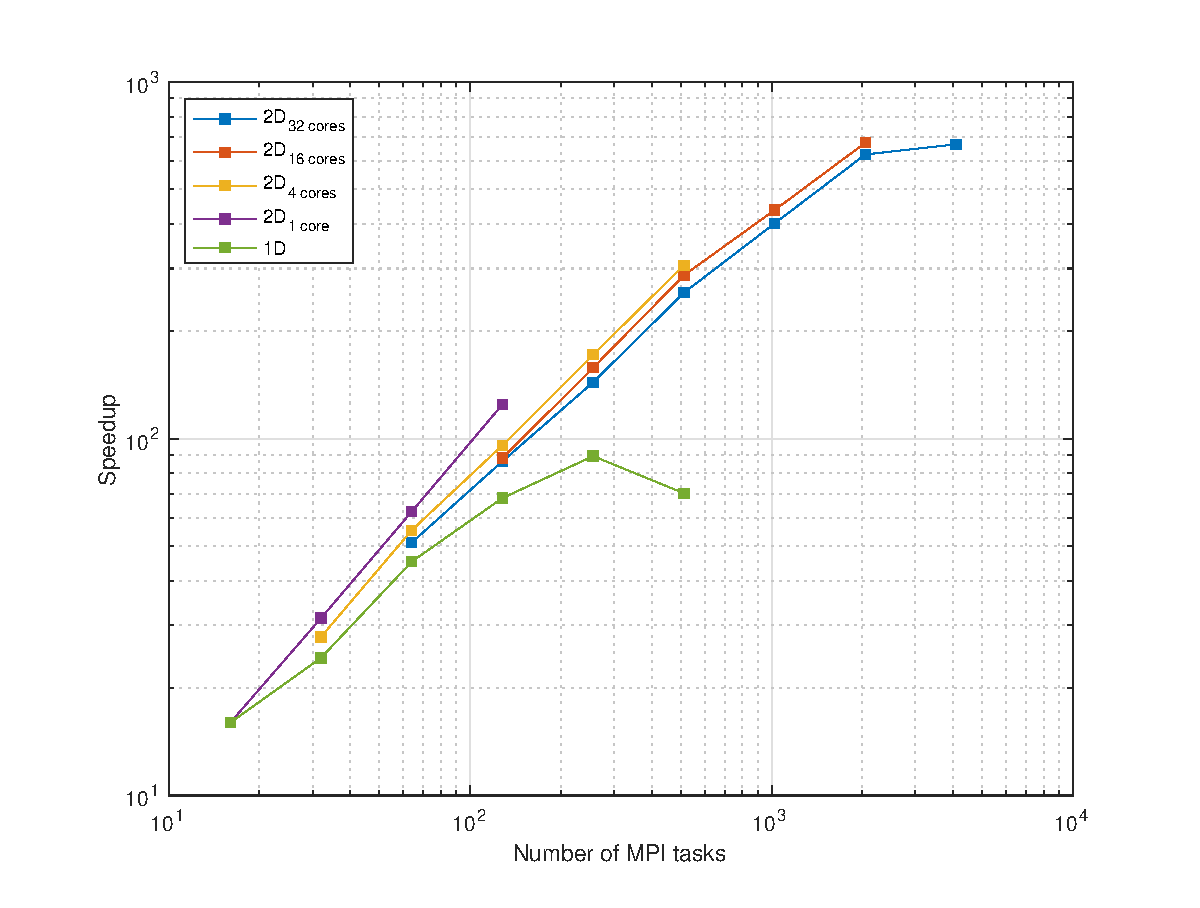
\includegraphics[scale=0.6]{grafici/20482}
\caption{Speedup factor of $4096\times512 \times256$ simulation}
\label{20482}
\end{center}
\end{figure}





\section{Benchmarks conclusions}
The benchmark series has highlighted common trends present in our simulations.
\par
By looking at the curves, we can see that the performances envelope is bordered by the 64 cores run and the single core ones.  We can catch from the graphs that the code tends to perform faster using as less threads per processor as possible.  This behavior is reasonable, since our code and the library in which we rely on to perform the MPI transposition, does not implement the OpenMP technology at the moment, so, although we could carry on the simulation basing our communications on MPI, we will experience efficiency lacks when dealing with intra-node messagings. In particular, when dealing with many cores per processor we face a speedup tendency to pass from 2 to $2^{2/3}$, as the number of MPI tasks gets doubled, as highlighted in~\cite{dns:gpu:supercomputer}. \par
Unfortunately, the Intel KNL's architecture~\cite{intel:xeonphi} is designed to exploit code vectorization as much as possible and OpenMP plays a key role in this kind of implementations. \par
We suggest to move to traditional processors architectures, instead of using MIC, to experience lower losses. Our simulations in fact has highlighted that, although MPI can not guarantee high efficiency in heavily threaded applications, the lacks using 16 cores, or less, per processor can be acceptable.\\
\par
As the problem size grows, the optimal number of MPI tasks, to achieve the best speedup, grows. In fact, we passed from 512 parallel processes for a $128^{3}$ simulation to 2048 for a $512^{3}$ simulation. \par

\begin{figure}
\begin{center}
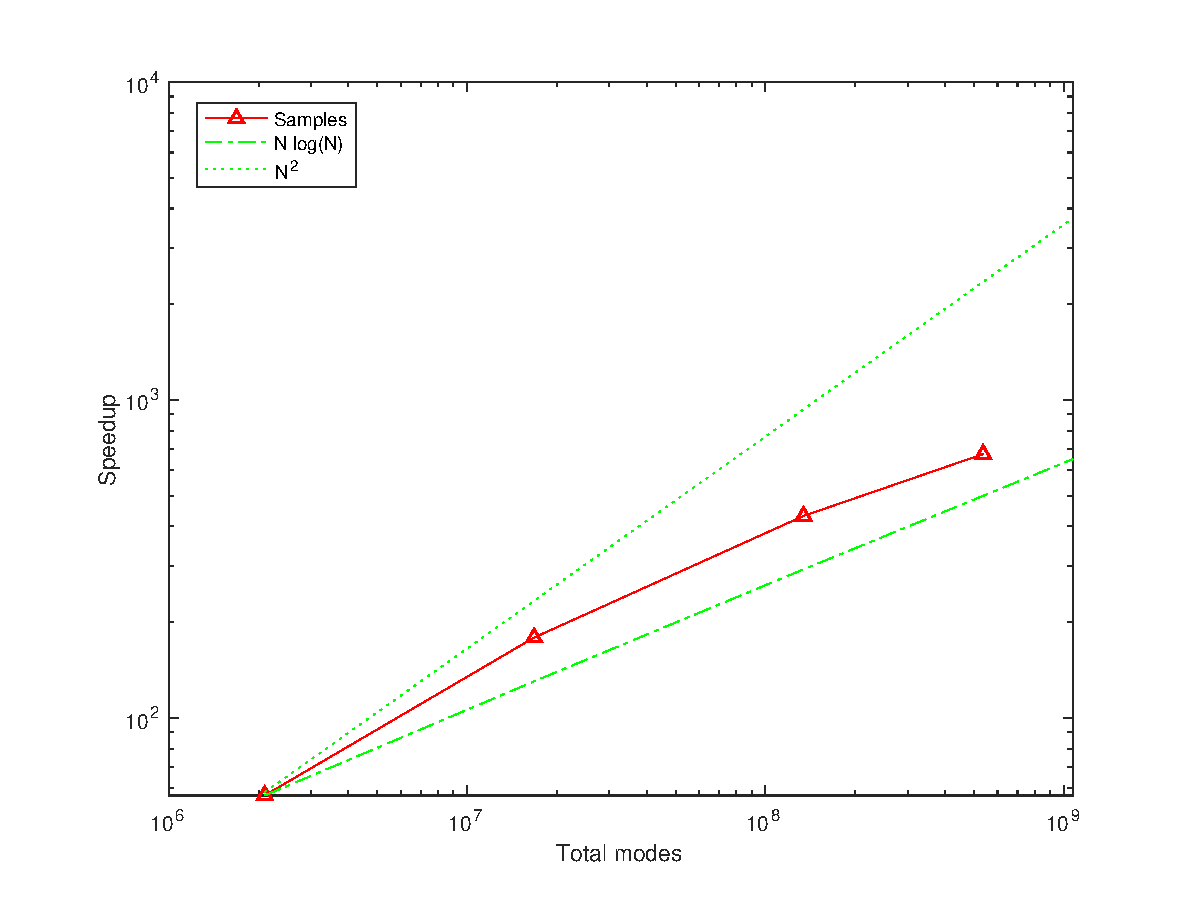
\includegraphics[scale=0.6]{grafici/speedup_trend}
\caption{Speedup factors growth}
\label{speedup:trend}
\end{center}
\end{figure}

On the other hand, the speedup factor increase its peak in a fashion which lies between $N\log(N)$ and $N^{2}$, like testify by figure~\ref{speedup:trend} in which our samples are plotted against such behaviors. \\
\par

Let us introduce the speedup comparison with hyper threading turned on. \par
Hyper threading is a technology developed by Intel~\cite{hyper:paper}  that virtually doubles the cores on the CPU, making the CPU run faster and more efficient by scheduling the workload between the cores. On modern Xeon Phi we can quadruplicate the number of cores, obtaining until 272 threads per processor. However, as our benchmark shows, this technology does not provide a boost in terms of speedup, on the contrary it penalizes our results in evident fashion.\par
In figure~\ref{hyper} are compared the original results of a $512^{3}$ simulation, running on different cores per processor, against two curves which exploit the hyper threading technology.\\
\par
In conclusion we would like to show the cost for a single degree of freedom (DOF) in terms of CPU time.
Such cost has been obtained considering the simulation time, the number of time steps required by the simulation and the total number of degrees of freedom, so it has to be intended as a mean value.
The cost is defined as:
\begin{equation}
Time/DOF = \frac{Sim Time}{timestep}\times \frac{1}{nx\times ny\times nz}
\end{equation}
Our results have been compared with the ones achieved in~\cite{Borrel}, where a boundary layer simulation is carried out on a flat plate, through direct numerical simulation, on JUGENE, a Blue Gene P architecture~\cite{blue:gene:chip}\cite{blue:gene:network} installed at Juelich Forschungszentrum, with its 32,768 cores.\par
Since the problems compared are just similar we can only obtain qualitative informations from that.

\begin{figure}
\begin{center}
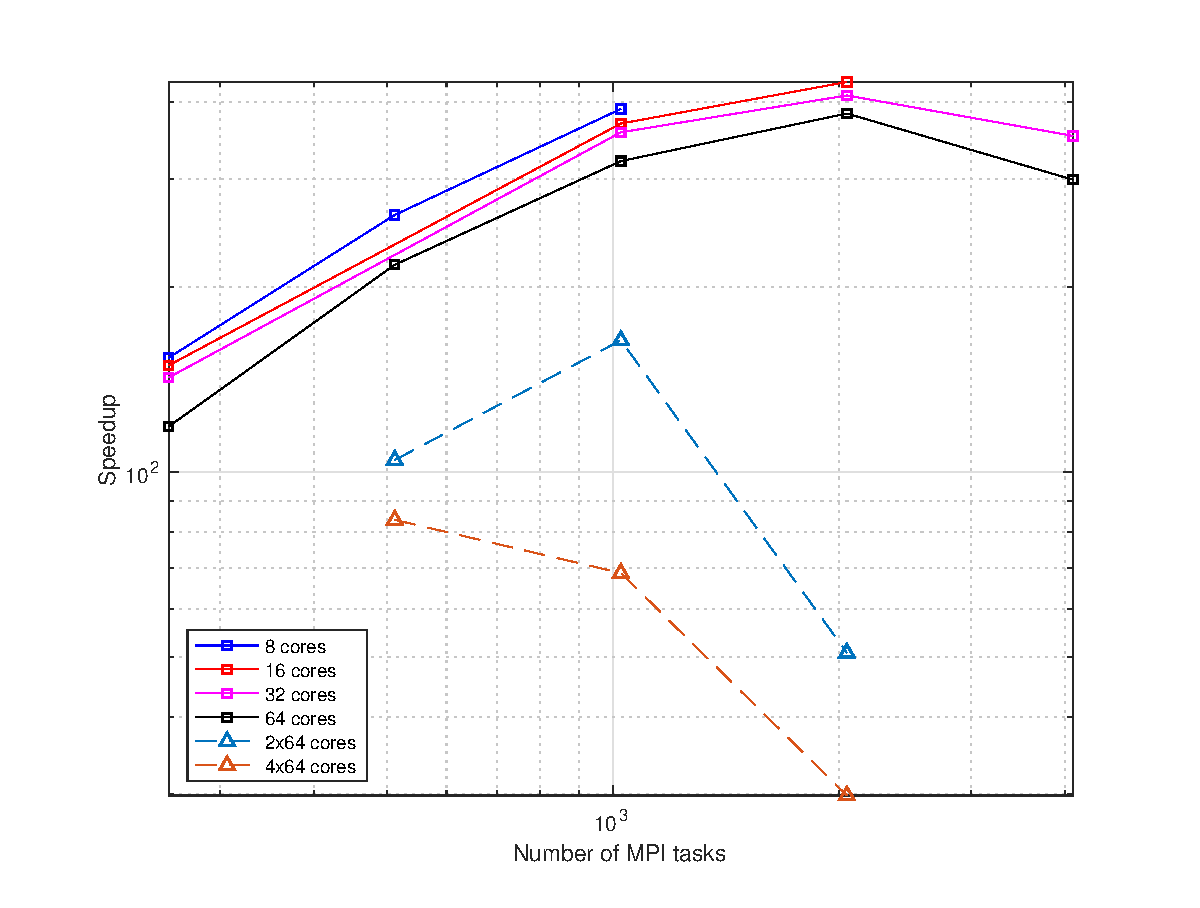
\includegraphics[scale=0.6]{grafici/hyperthreading}
\caption{Hyper threading benchmark}
\label{hyper}
\end{center}
\end{figure}

\begin{figure}
\begin{center}
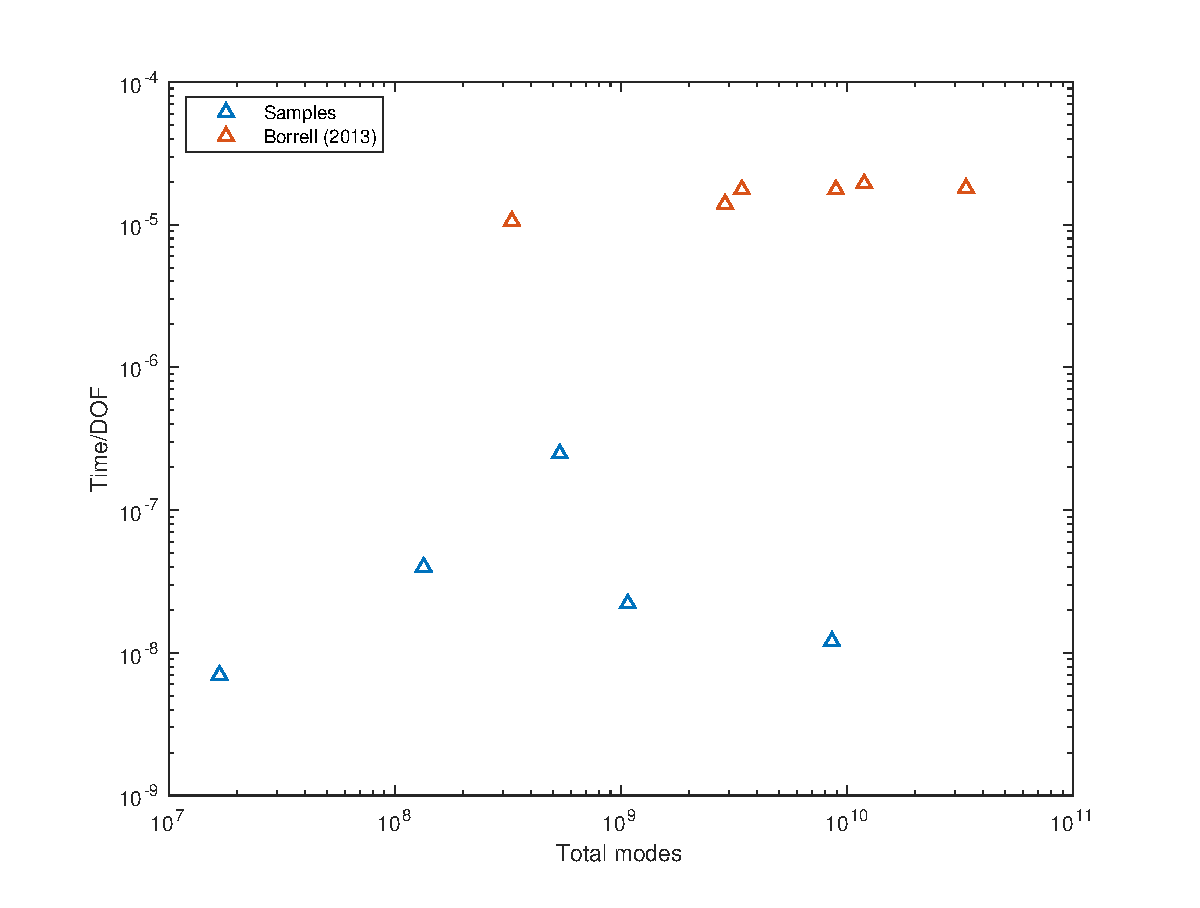
\includegraphics[scale=0.6]{grafici/time_dof}
\caption{Qualitative comparison of Time-DOF ratio}
\label{hyper}
\end{center}
\end{figure}


\backmatter
\addcontentsline{toc}{chapter}{\bibname} 
\printbibliography

\end{document}
